% 固定来源 PDF 印刷页 79 第 21 题评分解析构造线示意。
% 保留原解中 E、Q 与连接关系；投影不按比例。
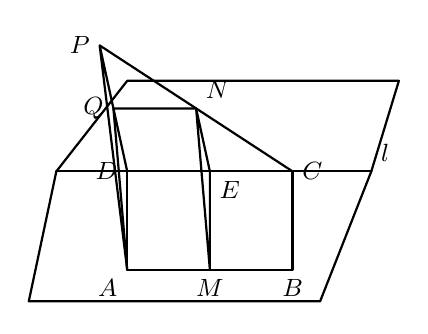
\begin{tikzpicture}[x=1cm,y=1cm,font=\small,line cap=round,line join=round]
  \coordinate (A) at (.7,-1.25); \coordinate (B) at (2.8,-1.25);
  \coordinate (D) at (.7,0); \coordinate (C) at (2.8,0);
  \coordinate (P) at (.35,1.6); \coordinate (M) at (1.75,-1.25);
  \coordinate (N) at (1.575,.8); \coordinate (E) at (1.75,0);
  \coordinate (Q) at (.525,.8);
  \draw[thick] (-.2,0)--(3.8,0);
  \draw[thick] (-.2,0)--(.7,1.15)--(4.15,1.15)--(3.8,0);
  \draw[thick] (-.2,0)--(-.55,-1.65)--(3.15,-1.65)--(3.8,0);
  \draw[thick] (A)--(B)--(C)--(D)--cycle;
  \draw[thick] (P)--(A) (P)--(C) (P)--(D);
  \draw[thick] (M)--(N) (N)--(E) (M)--(E) (A)--(Q) (N)--(Q);
  \draw[dashed] (Q)--(D);
  \node[left] at (P) {$P$}; \node[below left] at (A) {$A$};
  \node[below] at (B) {$B$}; \node[right] at (C) {$C$}; \node[left] at (D) {$D$};
  \node[below] at (M) {$M$}; \node[above right] at (N) {$N$};
  \node[below right] at (E) {$E$}; \node[left] at (Q) {$Q$};
  \node[above right] at (3.8,0) {$l$};
\end{tikzpicture}
